\documentclass[border=3mm]{article}

\usepackage{tikz}
\usepackage{qtree}
\usetikzlibrary{arrows,shapes.gates.logic.US,shapes.gates.logic.IEC,calc}
\begin{document}
\thispagestyle{empty}
\tikzstyle{branch}=[fill,shape=circle,minimum size=3pt,inner sep=0pt]
\begin{tikzpicture}[label distance=2mm]

    \node (x3) at (0,0) {$x_3$};
    \node (x2) at (1,0) {$x_2$};
    \node (x1) at (2,0) {$x_1$};
    \node (x0) at (3,0) {$x_0$};

    \node[not gate US, draw, rotate=-90] at ($(x2)+(0.5,-1)$) (Not2) {};
    \node[not gate US, draw, rotate=-90] at ($(x1)+(0.5,-1)$) (Not1) {};
    \node[not gate US, draw, rotate=-90] at ($(x0)+(0.5,-1)$) (Not0) {};

    \node[or gate US, draw, logic gate inputs=nnn] at ($(x0)+(2,-2)$) (Or1) {};
    \node[or gate US, draw, logic gate inputs=nnnn] at ($(Or1)+(0,-1)$) (Or2) {};
    \node[or gate US, draw, logic gate inputs=nnn] at ($(Or2)+(0,-1)$) (Or3) {};
    \node[xor gate US, draw, logic gate inputs=nn] at ($(Or3)+(0,-1)$) (Xor1) {};
    \node[and gate US, draw, logic gate inputs=nn, anchor=input 1] at ($(Or3.output)+(1,0)$) (And1) {};
    \node[nor gate US, draw, logic gate inputs=nn, anchor=input 1] at ($(Or2.output -| And1.output)+(1,0)$) (Nor1) {};
    \node[and gate US, draw, logic gate inputs=nn, anchor=input 1] at ($(Or1.output -| Nor1.output)+(1,0)$) (And2) {};

    \foreach \i in {2,1,0}
    {
        \path (x\i) -- coordinate (punt\i) (x\i |- Not\i.input);
        \draw (punt\i) node[branch] {} -| (Not\i.input);
    }
    \draw (x3) |- (Or2.input 1);
    \draw (x3 |- Or1.input 1) node[branch] {} -- (Or1.input 1);
    \draw (x2) |- (Xor1.input 1);
    \draw (x2 |- Or3.input 1) node[branch] {} -- (Or3.input 1);
    \draw (Not2.output) |- (Or2.input 2);
    \draw (x1) |- (Or3.input 2);
    \draw (x1 |- Or1.input 2) node[branch] {} -- (Or1.input 2);
    \draw (Not1.output) |- (Xor1.input 2);
    \draw (Not1.output |- Or2.input 3) node[branch] {} -- (Or2.input 3);
    \draw (x0) |- (Or2.input 4);
    \draw (Not0.output) |- (Or3.input 3);
    \draw (Not0.output |- Or1.input 3) node[branch] {} -- (Or1.input 3);
    \draw (Or3.output) -- (And1.input 1);
    \draw (Xor1.output) -- ([xshift=0.5cm]Xor1.output) |- (And1.input 2);
    \draw (Or2.output) -- (Nor1.input 1);
    \draw (And1.output) -- ([xshift=0.5cm]And1.output) |- (Nor1.input 2);
    \draw (Or1.output) -- (And2.input 1);
    \draw (Nor1.output) -- ([xshift=0.5cm]Nor1.output) |- (And2.input 2);
    \draw (And2.output) -- ([xshift=0.5cm]And2.output) node[above] {$f_1$};

\end{tikzpicture}







\tikzstyle{branch}=[fill,shape=circle,minimum size=3pt,inner sep=0pt]
\begin{tikzpicture}[label distance=2mm]
    % nodes
    \node (x) at (-1,6) {$x$};
    \node (y) at ($(x) + (0,-1.2)$) {$y$};
    \node[not gate US, draw] at ($(x)+(0.5,-0.8)$) (notx) {};
    \node[not gate US, draw] at ($(y)+(0.5,-0.8)$) (noty) {};
    \node[and gate US, draw, rotate=-90, logic gate inputs=nn] at (1,3) (A) {};
    \node[and gate US, draw, rotate=-90, logic gate inputs=nn] at ($(A)+(2,0)$) (B) {};
    \node[and gate US, draw, rotate=-90, logic gate inputs=nn] at ($(B)+(2,0)$) (C) {};
    \node[or gate US, draw, rotate=-90, logic gate inputs=nn] at ($(A)+(1,-1.5)$) (D) {};
    % draw NOT nodes
    \foreach \i in {x,y} {
        \path (\i) -- coordinate (punt\i) (\i |- not\i.input);
        \draw (\i) |- (punt\i) node[branch] {} |- (not\i.input);
    }
    % direct inputs
    \draw (puntx) -| (C.input 1);
    \draw (punty) -| (C.input 2);
    \draw (puntx) -| (B.input 1);
    \draw (punty) -| (A.input 2);
    \draw (notx) -| (A.input 1);
    \draw (noty) -| (B.input 2);
    \draw (A.output) -- ([yshift=-0.2cm]A.output) -| (D.input 2);
    \draw (B.output) -- ([yshift=-0.2cm]B.output) -| (D.input 1);
    \draw (C) -- ($(C) + (0, -1.8)$) -- node[right]{$R$} ($(C) + (0, -2.5)$);
    \draw (D.output) -- node[right]{$U$} ($(D) + (0, -1)$);
\end{tikzpicture}





\Tree [.a [.f [.g [.b c ] [.h i ] ] ] [.e j ] ]




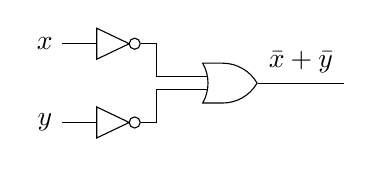
\begin{tikzpicture}
    \node (x) at (0, 1) {$x$};
    \node (y) at (0, 0) {$y$};

    \node[not gate US, draw] at ($(x) + (0.8, 0)$) (notx) {};
    \node[not gate US, draw] at ($(y) + (0.8, 0)$) (noty) {};
    \node[or gate US, draw, rotate=0, logic gate inputs=nn] at ($(noty) + (1.5, 0.5)$) (xory) {};

    \draw (x) -- (notx.input);
    \draw (y) -- (noty.input);

    \draw (notx.output) -- ([xshift=0.2cm]notx.output) |- (xory.input 1);
    \draw (noty.output) -- ([xshift=0.2cm]noty.output) |- (xory.input 2);

    \draw (xory.output) -- node[above]{$\bar x + \bar y$} ($(xory) + (1.5, 0)$);
\end{tikzpicture}








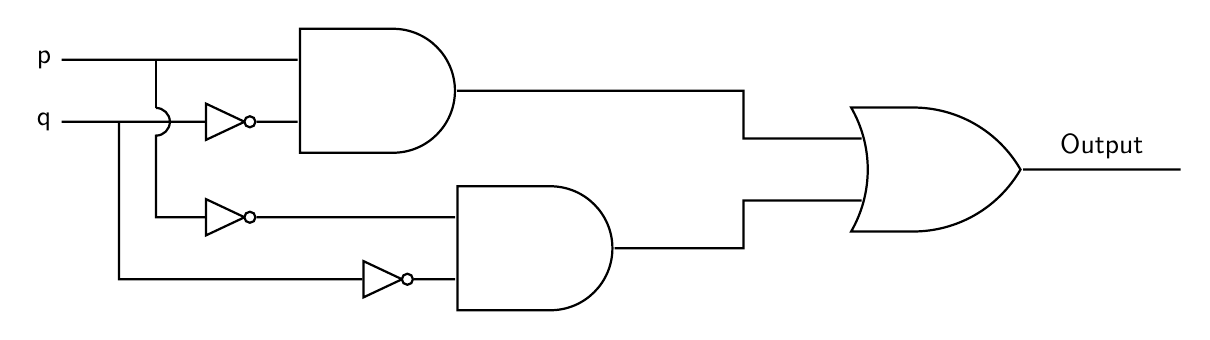
\begin{tikzpicture}[
        %Environment config
        font=\sffamily,
        thick,
        %Environment styles
        GateCfg/.style={
            logic gate inputs={normal,normal,normal},
            draw,
            scale=2
        }
    ]
    \path
        (0,0) node[and gate US,GateCfg](AND1){} 
            ++ (2,-2) node[and gate US,GateCfg](AND2){} 
            ++ (5,1) node[or gate US,GateCfg](OR1){}
        (AND1.input 3)
            ++ (-1,0) node[not gate US, draw](N1){}
        (AND2.input 3)
            ++ (-1,0) node[not gate US, draw](N2){}
        (AND2.input 1 -| N1)
            node[not gate US, draw](N3){};

    \draw
        (OR1.input 1) -- ++(-1.5,0) |- (AND1.output)
        (OR1.input 3) -- ++(-1.5,0) |- (AND2.output)
        (N2.output)--(AND2.input 3)
        (N1.output)--(AND1.input 3)
        (N3.output)--(AND2.input 1)
        (AND1.input 1) 
            -- ++(-3,0) coordinate (init) node[anchor=east]{p}
            node[pos=0.6](temp){}
        (N1-| temp)
            ++(0,5pt) edge (temp.center)
            arc (90:-90:5pt) |- (N3.input)
        (init |- N1) node[anchor=east]{q} 
            -- (N1.input) node[pos=0.4](temp2){}
        (temp2.center) |- (N2.input)
        (OR1.output) -- ++(2,0) node [midway,anchor=south]{Output};
\end{tikzpicture} 
    
    
    
    



\tikzstyle{branch}=[fill,shape=circle,minimum size=2pt,inner sep=0pt]
\begin{tikzpicture}[label distance=2mm]

\node (A) at (0, 0) {\small{A}};

\node (B) at (0, -1) {$B$};
\node (C) at (0, -2) {$C$};

\node[xor gate US, draw, anchor=input 1] at ($(A) + (2, 0)$) (xor1) {};
\node[xor gate US, draw, anchor=input 1] at ($(B) + (2, 0)$) (xor2) {};
\node[nand gate US, draw, anchor=input 1] at ($(xor1.output) + (2, -0.25)$) (nand1) {};
\node[nand gate US, draw, anchor=input 1] at ($(xor2.output) + (2, -0.25)$) (nand2) {};
\node[nand gate US, draw, anchor=input 2] at ($(nand2.output) + (2, 0)$) (nand3) {};
\node[xor gate US, draw, anchor=input 1] at ($(nand3.output) + (1, 0)$) (xor3) {};
\node[nand gate US, draw, anchor=input 1] at ($(C) + (2, -0.5)$) (nand4) {};
\node[nand gate US, draw, anchor=input 1] at ($(C) + (2, -1.5)$) (nand5) {};
\node[nand gate US, draw, anchor=input 1] at ($(C) + (2, -2.5)$) (nand6) {};
\node[nand gate US, draw, anchor=input 1] at ($(nand4.output) + (2, -0.5)$) (nand7) {};
\node[nand gate US, draw, anchor=input 2] at ($(nand7.output) + (2, -0)$) (nand8) {};
\node[nand gate US, draw, anchor=input 1] at ($(nand8.output) + (1, -1)$) (nand9) {};
\node (V) at ($(xor1.input 2) - (2, 0)$) {\small{$V_{cc}$}};

\node (D) at ($(xor3.output) + (1, 0)$) {D};
\node (E) at ($(nand9.output) + (1, 0)$) {E};


\draw (A) |- (xor1.input 1);
\draw (A) -- ($(A) + (1.5, 0)$) node[branch] {} -- ($(nand6.input 1) + (-0.5, 0)$) -- (nand6.input 1);
\draw ($(A) + (1.5, -1.5)$) node[branch] {} -- ($(nand2.input 2) + (-2, 0)$) -- (nand2.input 2);
\draw ($(nand4.input 1) - (0.5, 0)$) node[branch] {} -- (nand4.input 1);
\draw (V) -- (xor1.input 2);
\draw ($(V) + (1, 0)$) node[branch] {} -- ($(xor2.input 2) - (1, 0)$) -- (xor2.input 2);
\draw ($(xor2.input 2) - (1, 0)$) node[branch] {} -- ($(nand4.input 2) - (1, 0)$) -- (nand4.input 2);
\draw ($(nand4.input 2) - (1, 0)$) node[branch] {} -- ($(nand5.input 1) - (1,0)$) -- (nand5.input 1);
\draw (B) -- (xor2.input 1);
\draw ($(B) + (0.5, 0)$) node[branch] {} -- ($(nand1.input 2) - (4.23, 0)$) -- (nand1.input 2);

\draw (xor1.output) -- ([xshift=0.5cm]xor1.output) |- (nand1.input 1);
\draw (xor2.output) -- ([xshift=0.5cm]xor2.output) |- (nand2.input 1);
\draw (nand2.output) -- (nand3.input 2);
\draw (nand1.output) -- ([xshift=0.5cm]nand1.output) |- (nand3.input 1);
\draw (nand3.output) |- (xor3.input 1);
\draw (C) -- ([xshift=0.5cm]C) |- ([xshift=-0.5cm, yshift=-0.5cm]xor3.input 2) |- (xor3.input 2);
\draw ($(C) + (7, 0)$) node[branch] {} |- (nand8.input 1);
\draw (nand7.output) |- (nand8.input 2);
\draw (nand4.output) -- ([xshift=0.5cm]nand4.output) |- (nand7.input 1);
\draw (nand5.output) -- ([xshift=0.5cm]nand5.output) |- (nand7.input 2);
\draw (nand8.output) -- ([xshift=0.5cm]nand8.output) |- (nand9.input 1);
\draw (nand6.output) -- ([xshift=0.5cm]nand6.output) |- (nand9.input 2);
\draw (xor3.output) -- (D);
\draw (nand9.output) -- (E);


\end{tikzpicture}







\end{document} 